\chapter{Maximum and Minimum of Multivariable Functions}
For a $C^3$ function (in a neighborhood of $a$ in $\bbR$), by Taylor's Theorem $$f(a+h)=f(a)+f'(a)h+\frac12f''(a)h^2+\underbrace{\frac16f'''\lt(\begin{tabular}{c}\text{some point}\\ \text{between}\\ $a$ \text{ and } $a+h$\end{tabular}\rt)h^3}_{\substack{ \text{Remainder term }r(h) \\ \frac{r(h)}{h^2}\to 0 \text{ as }h\to 0}}$$Suppose $f'(a)=0$ ``$a$ is a critical point of $f$". Then
$$\frac{f(a+h)-f(a)}{h^2}=\frac12f''(a)+\frac{r(h)}{h^2}$$
If $f''(a)>0$ then $f$ has a local minimum at $a$ because choose $\delta >0$  such that $|h|<\delta$, $\lt|\frac{r(h)}{h^2}\rt|<\frac12f''(a)$. Then $RHS>0$ $\forall \ h$ such that $|h|<\delta$ and so for $h\in (-\delta,\delta)$, $f(a+h)>f(a)$ i.e. $f(a)$ is minimum value of $f$ in the neighborhood $(a-\delta,a+\delta)$. Similarly $f''(a)<0$ then $f$ has  a local maximum  at $a$. 


We want to find an analogy  of this for multivariable case

$f:(\text{open }U\text{ in }\bbR^n )\to \bbR$ a $C^3$ function. Then  for $h\in $ some  open neighborhood $W$ of origin, $a+h\in U$ \begin{align*}
	f(a+h) & =f(a)+f'(a)h+\frac12f''(a)(h,h)+\underbrace{\frac16f'''\lt(\begin{tabular}{c}
		  \text{some point}    \\
		    \text{between}     \\
		$a$ \text{ and } $a+h$
	\end{tabular}\rt)(h,h,h)}_{\substack{ \text{Remainder term }r(h) \\ \frac{r(h)}{h^2}\to 0 \text{ as }h\to 0}} \\
	& = f(a)+\lt[ \begin{matrix}
		D_1 & \cdots & D_n
	\end{matrix} \rt]\lt[ \begin{matrix}
	h_1\\ \vdots \\ h_n
\end{matrix} \rt]+\frac12 \sum_{i,j}D_iD_jf(a)h_ih_j+r(h)\\
&=  f(a)+\lt[ \begin{matrix}
	D_1 & \dots & D_n
\end{matrix} \rt]\lt[ \begin{matrix}
	h_1\\ \vdots \\ h_n
\end{matrix} \rt] +\frac12 \lt[ \begin{matrix}
h_1& \cdots & h_n
\end{matrix}\rt][D_iD_jf(a)] \lt[ \begin{matrix}
h_1\\ \vdots\\ h_n
\end{matrix} \rt]+r(h)\\
&=f(a)+\nabla f(a)\cdot h+\frac12 h^T \underbrace{[D_iD_jf(a)]}_{\substack{\text{Hessian Matrix}\\ \text{of }f\text{ at }a}}h+r(h)
\end{align*}
\dfnc{Hessian Matrix of $f$}{
	Let $f:(\text{open }U\text{ in }\bbR^n )\to \bbR$ such that $\begin{cases}
		f\text{ is }C^1\iff \deld{f}{x_i}\text{ are not continuous on }U\\
		f'' \text{ exists at }a
	\end{cases}$ So components of $f''$ are $D_iD_jf(a)$. Hessian of $f$ at $a$ = Square matrix $[D_iD_jf(a)]$
}
When $f$ is $C^2$, Hessian matrix is Symmetric Matrix

\dfnc{Critical Point}{
Let $f$ be a $C^1$ function, Open $U$ in $\bbR^n\xrightarrow{f}\bbR$. $a\in U$ is called critical point if $f'(a)=0\iff \nabla f(a)=0$
}
If $f$ has local maximum  at $a$, then along any line through $a$ the same must be hold, so all directional derivative =0 at $a$.
\dfnc{Non-degenerate Point}{If $f$ is $C^2$  then a critical point $a$  is called non-degenerate if the Hessian, $Hf(a)$ is non-singular i.e. $\det(Hf(a))\neq 0$
}

\begin{Claim}{}{}
	Symmetric Matrix  $A$ is positive (semi)definite $\iff $ $\forall$ nonzero vector $x\in \bbR^n$, $x^TAx>0$ (resp. $\geq 0$)
\end{Claim}
\begin{proof}
	\subsubsection*{If Part:}
	$x=\sum\limits_{i}c_iv_i$. Where $v_i$ is the eigen-basis. Then \begin{align*}
		x^TAx & = \lt(\sum\limits_{i}c_iv_i\rt)^TA\lt(\sum\limits_{j}c_jv_j\rt) = \lt(\sum\limits_{i}c_iv_i\rt)^T\lt( \sum_j\lm_jc_jv_j \rt) = \sum_i\lm_ic_i^2>0 \qquad [v_i^Tv_j=\delta_{ij}]
	\end{align*}
\subsubsection*{Only If Part:}
Use $x^TAx>0$  for $x=v_i$ eigenvector $<0,$ $v_i^TAv_i=v_i\lm_iv_i=\lm_i$
\end{proof}
\nt{Determinant of positive definite matrix $>0$ and Determinant of negative definite matrix has sign $(-1)^n$}



\begin{theorem}{}{maxminif}
Let $f:(\text{open }U\text{ in }\bbR^n )\to \bbR$. Suppose $f $ has a local maximum or minimum  at $a$  then \begin{enumerate}[label=\bfseries\tiny\protect\circled{\small\arabic*}]
	\item If $f'(a)$ exists then $f'(a)=0$ i.e. $a$ is a critical point. 
	\item Suppose in addition to that $f''(a)$  exists then if $f$ has local maximum at $a$, then $f''(a)\leq 0$ and if $f$ has local minimum at $a$, then $f''(a)\geq 0$
\end{enumerate}
\end{theorem}
\begin{proof}
	\begin{enumerate}[label=\bfseries\tiny\protect\circled{\small\arabic*}]
		\item For $n=1$  let we have local minimum at $a$. Then for small $|h|$
		
		\begin{center}
			 $\begin{rcases}
			 	\frac{f(a+h)-f(a)}{h}\geq 0 & \text{ for }h>0 \\
			 	\frac{f(a+h)-f(a)}{h}\leq 0 & \text{ for }h<0
			 \end{rcases}$Thus imply respectively that $f'(a)$  must be $\geq 0$ and $\leq 0$
		\end{center}
	For $n>1$  use $n=1$ in every direction i.e. for function $\lt. f\rt|_{a+tv}$ for $t\in $ open interval  to conclude $D_vf(a)=0$ $\forall$ directions. So $f'(a)=0$\Qed
	\item For $n=1$ $$f''(a)=\lim\limits_{h\to 0}\frac{f'(a+h)-f'(a)}{h}=\lim\limits_{h\to 0}\frac{f'(a+h)}{h}$$ 
	\parinf 
	
	\textbf{\textit{Observation: }}If $f$ has local maximum at $a$ then for $0<|h|<\delta$, $f(a+h)\geq f(a)$. So by $MVT$  there is $k$ between $0$ and $h$  such that $$\frac{f(a+h)-f(a)}{h}=f'(a+k)$$\parinn
	
	Using the observation $f''(a)=\lim\limits_{h\to 0}\frac{f'(a+k)}{h}\geq 0$
	
	For $n>1$ applying this  to each $\lt. f\rt|_{a+tv}$ $\forall$ direction vectors $v$  we get all $D^2_vf(a)\geq 0$. In terms of Hessian  let $v=\sum c_ie_i\implies D_vf=\sum c_iD_if\implies D^2f(a)=\sum_{i,j}c_jc_iD_jD_if(a) $ in  a neighborhood of $a$. $$D^2_vf(a)=\lt[ \begin{matrix}
		c_1 & \cdots & c_n
	\end{matrix} \rt]Hf(a)\lt[ \begin{matrix}
	c_1\\ \vdots\\ c_n
\end{matrix} \rt]$$
	\end{enumerate}
\end{proof}

\begin{theorem}{}{}
If $f:(\text{open }U\text{ in }\bbR^n )\to \bbR$ is a $C^3$  function  and $a$ is a non-generate critical point  of $f$  then 



\begin{center}
	\begin{tabular}{rcl}
		$f$ has a local minimum at $a$ & $\iff$ & $H$ is positive definite            \\
		                               & $\iff$ & All eigenvalues of $H$ are positive \\
		$f$ has a local maximum at $a$ & $\iff$ & $H$ is negative definite            \\
		                               & $\iff$ & All eigenvalues of $H$ are negative \\
		$f$ has saddle-point otherwise &        & $H$ is indefinite
	\end{tabular}
\end{center}
\end{theorem}
\begin{proof}
	\subsubsection*{If Part:}
	We already proved the if direction in \hyperref[th:maxminif]{Theorem \ref{th:maxminif}}
	
	\subsubsection*{Only If Part:}
	By Taylor's theorem $$f(a+x)-f(a)=\cancelto{0}{f’(a)}x+\frac12x^THx+r(x)$$with as $\|x\|\to 0$, $\frac{r(x)}{\|x\|^2}\to 0$. Let's assume that $H$ is positive definite. So far $x\neq 0$ and $x^THx>0$. 
	The function $x\to x^THx$ is continuous, so on the compact set $\{u\mid \|u\|=1\}$ it is bounded and achieves its infimum $\mu$. So $\mu>0$ So $$\frac{x^THx}{\|x\|^2}\geq \mu\ \forall \ x\neq 0\implies \lt(\frac{x}{\|x\|}\rt)^TH\lt( \frac{x}{\|x\|} \rt)$$ Since $\frac{r(x)}{\|x\|^2}\to 0$ as $\|x\|\to 0$, we can find $\delta>0$ such that $\frac{|r(x)|}{\|x\|^2}<\frac{\mu}{2}$ when $\|x\|<\delta$. Thus for $\|x\|<\delta$ we have $f(a+x)-f(a)\geq 0$ i.e. $f$ has a local minimum at $a$
\end{proof}

\dfnc{Saddle Point}{At  a nondegenrate critical point $a$, $H$ has both \begin{center}
		\begin{tabular}{c}
		$a$ positive eigenvalue, say $\lm_1$ with eigen vector $u_1$\\
		$a$ negative eigenvalue, say $\lm_2$ with eigen vector $u_2$
\end{tabular}
	\end{center}This means $D^2_{u_1}f(a)>0$, so in the $u_1$ direction $f$ has local minimum and $D^2_{u_2}f(a)<0$, so in the $u_2$ direction $f$ has local maximum

\begin{center}
	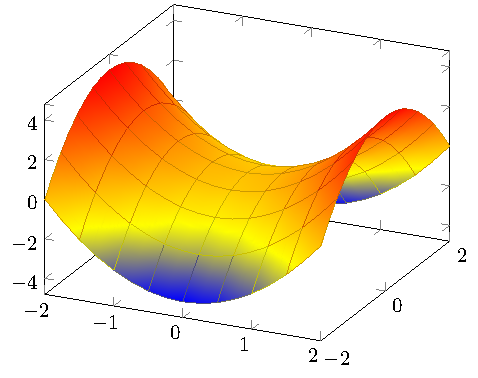
\includegraphics[width=6cm]{images/saddle.pdf}
\end{center}
}
\exc{}{Many times functions are $C^{\infty}$ whenever defined so all of the above applies.\begin{itemize}
		\item $f(x,y)=c,$ constant. All derivatives are zero, $H$ is zero.
		\item $f(x,y)=ax+by+c$ linear, $(a,b)\neq (0,0).$ No critical points.
		\item $f(x,y)=$ quadratic.
		
		General case $(x_1,x_2,\dots,x_n)=x\in\bbR^n$ \begin{align*}
			\Phi(x) &  =\sum_{i=1}^na_{ii}x_i^2+\sum_{1\leq i<j\leq n}2a_{ij}x_ix_j+\sum_{i=1}^np_ix_i+r\\
			& = x^TAx+px+r\\
			& =\lt[ \begin{matrix}
				x_1 & \cdots & x_n
			\end{matrix} \rt]\lt[ \begin{matrix}
			a_{11} & \cdots & a_{1n}\\ \vdots & \ddots & \vdots\\ a_{n1} & \cdots & a_{nn}
		\end{matrix} \rt]\lt[ \begin{matrix}
		x_1 \\ \vdots \\ x_n
	\end{matrix} \rt]+\lt[ \begin{matrix}
	p_1 &\cdots & p_n
\end{matrix} \rt]\lt[ \begin{matrix}
x_1 \\ \vdots \\ x_n
\end{matrix} \rt]+r \quad [\text{where }a_{ij}=a_{ji}]
		\end{align*}
	Hence $D_i\Phi(x)=\sum_{j=1}^n a_{ij}x_j+p_i$, $D\Phi(x)=2Ax+p$.	Critical points: $x$ such that $2Ax_p=0$
	
	If $2A=H$ is nonsingular then there is an unique critical point, namely $x=-H^{-1}p$. Then this point is local minimum is $H$ is positive definite, local maximum id $H$ is negative definite and saddle point otherwise
	\end{itemize}

}